\documentclass[12pt]{article}

\usepackage[margin=1in]{geometry}

\usepackage{amsmath}
\usepackage{graphicx}

\usepackage{caption, subcaption, xcolor}

\graphicspath{{res/}}

\title{Lab 2}
\author{Lukas Finkbeiner}

\begin{document}

\maketitle

\begin{abstract}

\textcolor{red}{We need more narrative drive. Consider using powerful transition phrases}

We investigated the hyperfine hydrogen transition by calibrating our measurements to thermal noise and by averaging over many blocks of data taken in optimal time windows of the day. We investigated the speed of light using waveguides (\textcolor{red}{How do they work?}). Our Chi-Squared analysis is completely deficient because our data were taken too broadly to show noticeable inconsistencies.

This is a great place to have a to-do section, because I prefer to write abstracts at the end of the writing process.

\quad * Ask Professor about the permissions thing (page 3), to make sure there are no technical difficulties.

\textcolor{red}{Figure out how to make the section headers smaller. They are taking up far too much space.}

\end{abstract}

\section{Introduction and Background}

\quad \quad In the first of two experiments, we seek to observe the 21-cm HI line, at 1420.4 MHz. However, we want to look at frequencies better suited to our lab equipment. For example, our PicoScope has a maximum sampling rate of 62.5 MHz, so anything above 125 MHz would be aliased.

\begin{figure}
\centering
	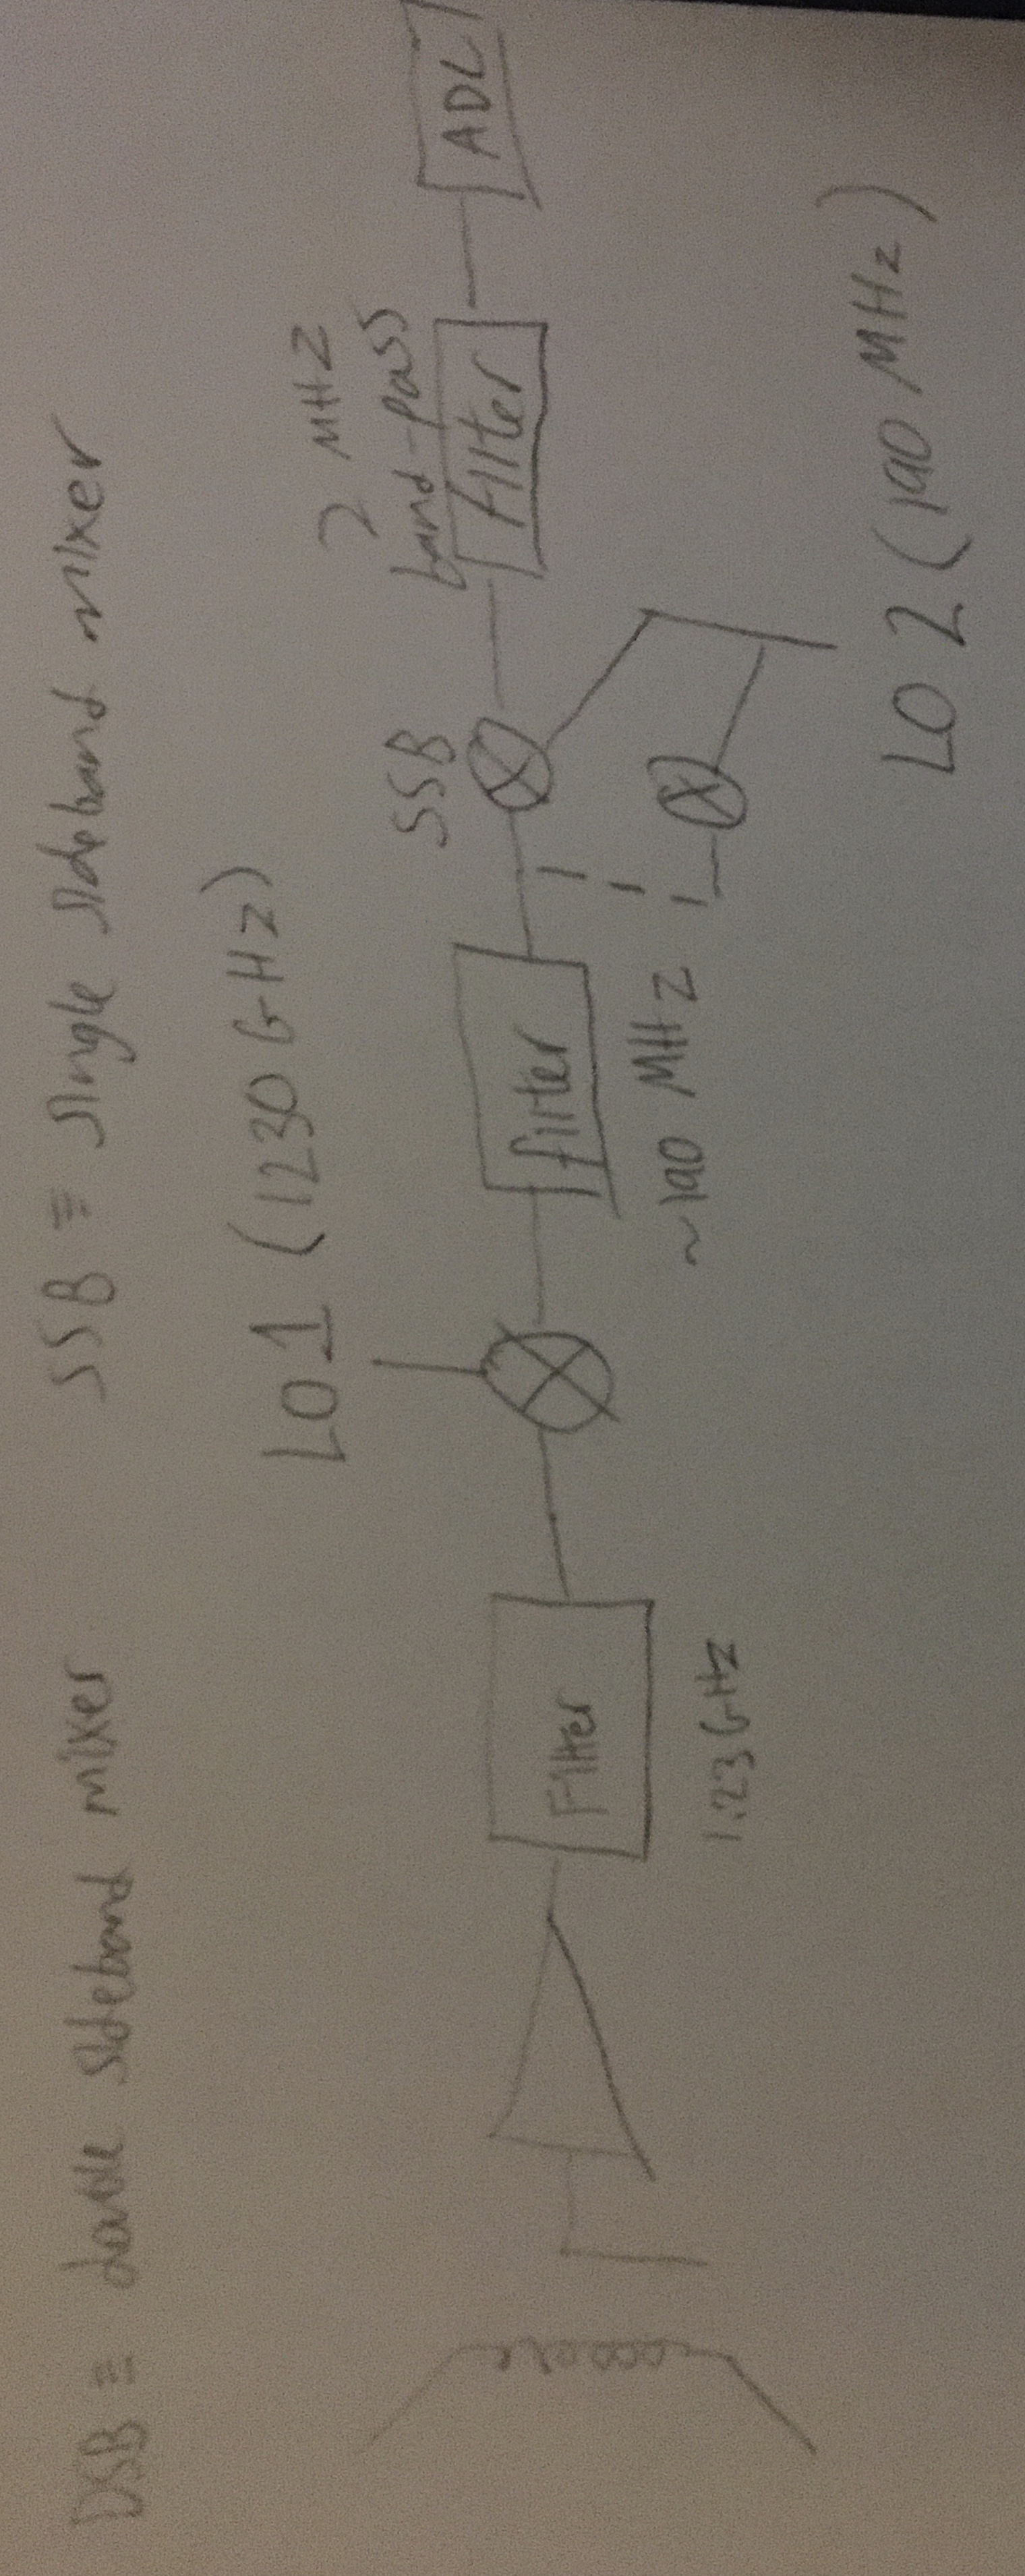
\includegraphics[angle=-90, width=.6\linewidth]{block}
	\caption{To reduce the frequencies of incoming signals to manageable levels, we employ a multi-stage combination of filters and mixers. The signal enters via transformer connected to the collector. The ADC represents the final step, when the PicoScope translates voltages over time into digital arrays.}
	\label{fig:block}
\end{figure}

The data that we sample from the Big Horn via the PicoScope will feature arbitrary units which depend on our setup. To calibrate the intensity of the spectrum, we first calculate the gain:

\begin{equation} \label{eq:thermal}
G = \frac{T_\text{sys, cal} - T_\text{sys, cold}}{\sum (s_\text{cal} - s_\text{cold})} \sum s_\text{cold} \approx \frac{\text{300 K}}{\sum (s_\text{cal} - s_\text{cold})} \sum s_\text{cold}
\end{equation}

Where $T_\text{sys, cal} \approx 98.6^\circ$ F $\approx 310$ K represents the temperature of the human flesh that we use to cover most of the telescope. $T_\text{sys, cold}$ represents the temperature of the cold sky. We expect $T_\text{sys, cold} \ll T_\text{sys, cal}$, whereby we get the approximated form on the right. $s_\text{cal}$ represents the spectrum for which we attempt to maximize thermal noise in the collector, and $s_\text{cold}$ represents the spectrum for which we attempt to minimize.

To remove constant sources of interference in our data and to obtain the shape of the line, we divide an `on' spectrum by an `off' spectrum. 

\begin{equation}
s_\text{line} = \frac{s_\text{on}}{s_\text{off}}
\end{equation}

The fully-calibrated spectrum represents a scaling of this $s_\text{line}$ by the thermal gain from equation \ref{eq:thermal}:

\begin{equation}
T_\text{line} = s_{line} \times G
\end{equation}

To plot our calibrated spectrum against Doppler velocity, we use the following relation:
\begin{equation}
v = -c \frac{\Delta \nu}{\nu_0}
\end{equation}

\textcolor{red}{I should probably enumerate the rotation matrices that I plan to use.}

For our second experiment, we seek to calculate to calculate the wavelength $\lambda_\text{sl}$ of a signal inside the waveguide based on the positions of the minima in the squared voltage, which we call nulls. We expect a linear dependence of null spacings on $\lambda_\text{sl}$. We use the following equation for this first experiment:

\begin{equation}
x_m = A + m \frac{\lambda_\text{sl}}{2}
\end{equation}

$m$ is the index of the null, $x_m$ is the position of null $m$, and $A$ represents a constant offset which can relate whether the far end of the waveguide is open or shorted.

The rectangular waveguide, to which we switch for the X-band phase of the experiment, abides a nonlinear relationship between the waveguide's width and the wavelengths of the input in the waveguide and in free space.

\begin{equation} \label{eq:xband}
\lambda_g = \frac{\lambda_\text{fs}}{[1 - (\frac{\lambda_\text{fs}}{2a})^2]^{1/2}}
\end{equation}

$\lambda_g$ is the guide wavelength, which we directly measure. $\lambda_\text{fs}$ is the free-space wavelength of the signal, which we will calculate using the known input frequency and the relation $c = f \lambda_\text{fs}$. $a$ is the width of the waveguide.

Finally, to analyze our results we define the reduced chi-squared function as follows:

\begin{equation}
\chi_r^2 = \frac{1}{N - M} \sum_i \frac{|y_i - \hat{y_i}|^2}{\sigma_i^2}
\end{equation}

Where $N$ is the number of data and $M$ is the number of fit parameters. For each measurement $i$, $y_i$ is the observed value, $\hat{y_i}$ is the value predicted by the fit, and $\sigma_i$ is the expected error on that measurement.

The reduced chi-squared function will provide something clear to minimize when fitting the data to a model. Specifically, we want to calculate the width $a$ based on our observations of null spacings, so we will calculate the value of $a$ which minimizes the reduced chi-squared.

\section{Methods}

%\textcolor{red}{Decide whether you will discuss this test signal.}
%To place our test signal in the upper and lower sidebands, we use these two frequencies. To put the hydgrogen in the upper and lower sidebands, we set the first local oscillator to these other two frequencies.

\quad \quad After setting the two local oscillators to 1230 and 190 MHz, as labeled in figure \ref{fig:block}, we set the power levels to 8 and 0 dBm, respectively. These numbers are difficult to theoretically justify; through trial and error, and particularly through consultation with other groups, we found that these numbers led to the greatest HI resolution for the Big Horn pointed directly upward.

However, these numbers changed when taking data for Cassiopeia, by which point our signal-to-noise ratio was too low. We switched to 10 dBm for both and proceeded with the pico-sampling at 62.5 / 6 MHz, the rate we used for all captures.

Later on, we will see imperfections in the setup in the form of nearly symmetric 'bunny ear' spikes as well as an extreme spike at the center; we found the PicoScope to sometimes artifically attenuate and offset the signal going into the second port, because we would switch the cables going into A and B and we would see the same shape; if there were a problem in our mixer stages, we would expect the output to switch similarly. 

We measure $\lambda_{sl}$ and its counterpart $\lambda_g$, the guide wavelengths, as the distance between the nulls in the guide output. We measure $a$ with a set of calipers and compare this with our results from a least-squares fit to the data based on equation \ref{eq:xband}.

\section{Observations}

% 1. initial calibration results. Here is a test signal. ``Our setup works!''
% source of error: angles are not aligned well. 10% error becomes... 25%? in power plot. I do not remember.

% scrap for time: justify the use of mean vs median. Actually, I simply lack a convenient graphical argument.
% what, then, is the difference between mean and median?

\quad \quad We collected data over many days of troubleshooting. The thermal data, as pictured in figure \ref{eq:thermal}, have a straightforward gap between them, but our gain calculation (of about 30) was well below that of other groups.

Other results surely point to some misunderstanding regarding the setup of the filters and mixer stages. Consider the rippling spikes which run along figure \ref{fig:on_limits}; the noise detracts from our results, and seems to vanish (at least, as a clear problem) when we raise the local oscillator power levels for the Cassiopeia measurements (the comparative smoothness will become obvious with the fully calibrated spectra in the analysis section). However, when we raised power levels for this initial HI line capture, the signal got drowned out somewhere.

\begin{figure}
	\centering
	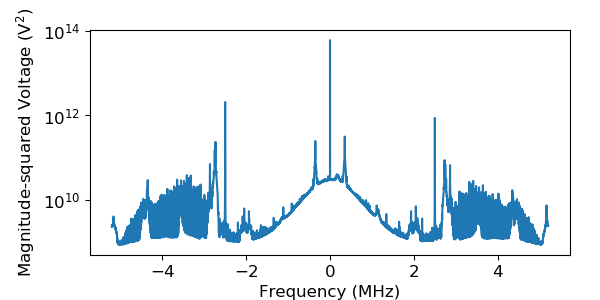
\includegraphics[width=.6\linewidth]{limits_justification}
	\captionof{figure}{A semi-log plot over the range of frequencies sampled. We assume that our 2 MHz low-pass filter works, so we will dismiss the signals farther than 2 MHz from the center. Additionally, the large central spike and smaller `bunny ear' spikes ($\pm$.5 MHz) appear on all data sets as persistent interference; we partially ignore these by limiting the y-axis.}
	\label{fig:on_limits}
\end{figure}

\begin{figure}
	\centering
	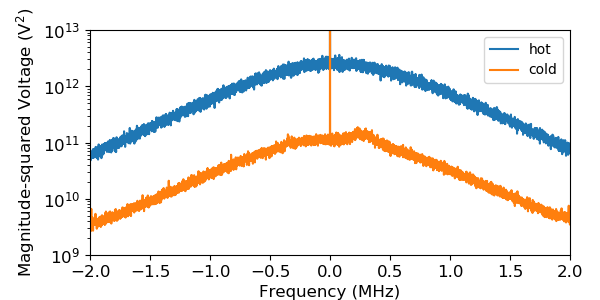
\includegraphics[width=.6\linewidth]{thermal}
	\captionof{figure}{The `hot' data correspond to three humans standing in front of the collector. The `cold' data correspond to the collector pointing up at the cold sky. The noise is not an issue, because it is regular: observe the even discrepancy between the curves over the domain of interest.}
	\label{fig:thermal}
\end{figure}

\begin{figure}
	\centering
	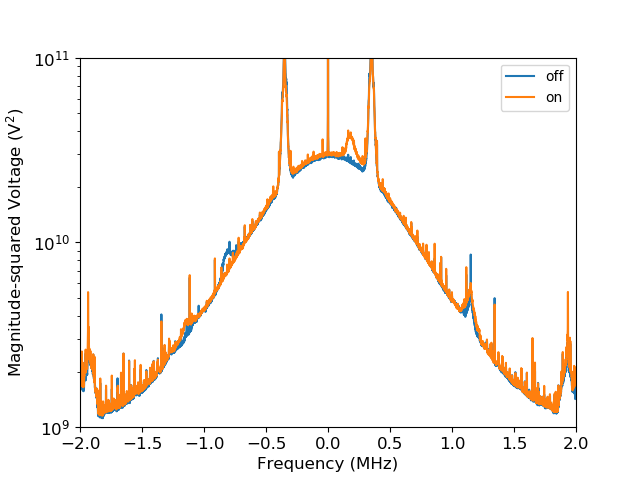
\includegraphics[width=.6\linewidth]{up_on_off}
	\caption{Combined plot of the `on' and `off' (LO1 at 1230 and 1231 MHz, respectively) power spectra. As we expect, the HI signal shifts by about 1 MHz between the two plots. This also supports our interpretation of the other patterns as interference: these patterns do not move between spectra.}
	\label{fig:up_on_off}
\end{figure}

% 4. Plot waveguide results?

% address VSWR, but it is a minor point

% caliper measurement for a. 'This is what we hope to get from analysis'
% sources of error.

\textcolor{red}{Bad need here for a transition}For the sake of brevity, we will plot the data for the 3GHz section later, in the analysis, along with the least-squares fit model.

Data from the XBand waveguide section, frequency and resulting null positions. All measurements come with an intrinsic reading error ($\pm .025$ cm) and, more importantly, poor resolution of the null's location. This poor resolution was partially due to variation in human judgment, but principally to the low signal-to-noise ratio. Near the null, the derivative of the magnitude-squared voltage with respect to waveguide slider position is at its most shallow. Consequently, there is a sort of range of positions over which the same null can be argued to appear. We decided that this uncertainty probably corresponds to a universal uncertainty of $\pm .2$ cm.

\begin{center}
 \begin{tabular}{||c c||} 
 \hline
 $f$ (GHz) & Null Positions (cm)\\ [0.5ex] 
 \hline
 7.0 & 8.8, 15.15 \\ 
 \hline
 7.2 & 11.95, 17.15 \\
 \hline
 7.5 & 10.05, 14.4 \\ 
 \hline
 8.0 & 10.15, 13.35, 16.7 \\
 \hline
 8.5 & 9.85, 12.7, 15.25 \\
 \hline 
 9.0 & 9.3, 12.3, 14.25, 16.7 \\ [1ex] 
 \hline
\end{tabular}
 \begin{tabular}{||c c||} 
 \hline
 $f$ (GHz) & Null Positions (cm)\\ [0.5ex] 
 \hline
 9.5 & 8.9, 11.15, 13.35, 15.45, 17.7 \\ 
 \hline
 10.0 & 8.45, 10.45, 12.3, 14.35, 16.5 \\
 \hline
 10.5 & 9.95, 11.75, 13.5, 15.45, 17.3 \\
 \hline
 11.0 & 9.35, 11.4, 12.65, 14.45, 16.2, 17.85 \\
 \hline
 11.5 & 8.95, 10.45, 12.0, 13.8, 15.15, 16.8 \\
 \hline
 12.0 & 8.4, 9.85, 11.35, 12.85, 14.4, 15.9, 17.45 \\ [1ex] 
 \hline
\end{tabular}
\end{center}

\section{Analysis}

\quad \quad Since the Horn was pointing straight up, we may say that the declination is equal to the latitude of the telescope. In our case, that is $37.873199^\circ \approx 0.661012$ radians. The right ascension is equal to the local sidereal time (LST) of data-capture.

We labeled all of our samples with unix time. Included below is a table including examples of date conversions to Doppler corrections for the events of interest. For the sake of brevity, we omit the counterparts for the Cassiopeia measurements.

\

\begin{center}
 \begin{tabular}{||c c c c||} 
 \hline
 Label & Unix Time & Julian Date & LST \\ [0.5ex] 
 \hline
 On-line start & 1582937209.9447305 & 2458908.5325225084 & 0.8334479646673989 \\ 
 \hline
 On-line stop & 1582937704.4486437 & 2458908.5382459336 & 0.8695077621535888 \\
 \hline
 Off-line start & 1582937837.5090616 & 2458908.5397859844 & 0.8792106794915676 \\
 \hline
 Off-line stop & 1582938387.1761112 & 2458908.5461478718 & 0.9192930359644231 \\ [1ex] 
 \hline
\end{tabular}
\end{center}

\begin{center}
 \begin{tabular}{||c c c||} 
 \hline
 Label & PST & Doppler Correction (m / s)\\ [0.5ex] 
 \hline
 On-line start & 2/28/20 @ 16:46:49 & -27648.19266498681 \\ 
 \hline
 On-line stop & 2/28/20 @ 16:55:04 & -27897.548197380296 \\
 \hline
 Off-line start & 2/28/20 @ 16:57:17 & -27960.009947759394 \\
 \hline
 Off-line stop & 2/28/20 @ 17:06:27 & -28197.027228226034 \\ [1ex] 
 \hline
\end{tabular}
\end{center}

\

The Doppler correction exhibits, at first glance, a critical time sensitivity. Observe that, just for one source (directly overhead), the final Doppler correction differed from the initial by about 550 m / s. However, as we shall soon see, the velocity axis will span many mega-meters, so taking the average of the Doppler corrections should suffice for a global correction.

\textcolor{red}{If I have extra space, put the results from the Cass. Doppler correction calculation}

\begin{figure}
	\centering
	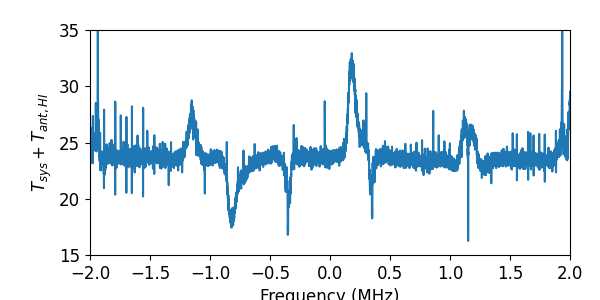
\includegraphics[width=.6\linewidth]{up_vs_frq}
	\caption{Here is a fully calibrated line. We see HI for sure!}
	\label{fig:up_vs_frq}
\end{figure}

\begin{figure}
	\centering
	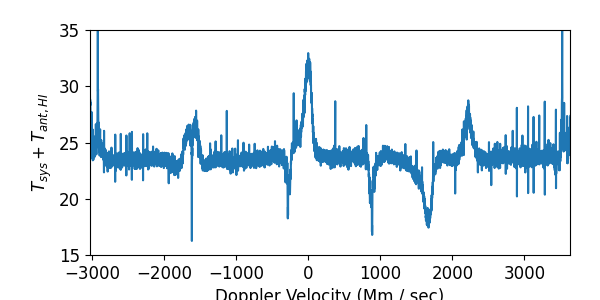
\includegraphics[width=.6\linewidth]{up_vs_vel}
	\caption{Here is that same line, now with a velocity axis. \textcolor{red}{What is the point I am trying to make with this plot?}}
	\label{fig:up_vs_vel}
\end{figure}

\begin{figure}
\centering
	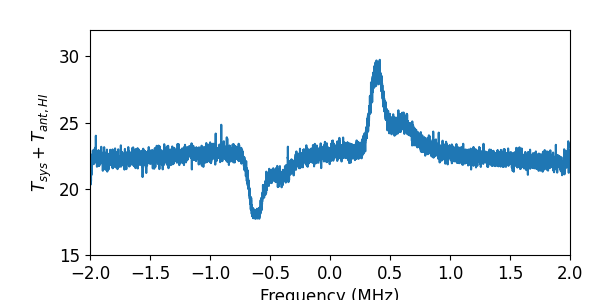
\includegraphics[width=.6\linewidth]{cass_vs_frq}
	\caption{...}
	\label{fig:cass_vs_frq}
\end{figure}

\begin{figure}
	\centering
	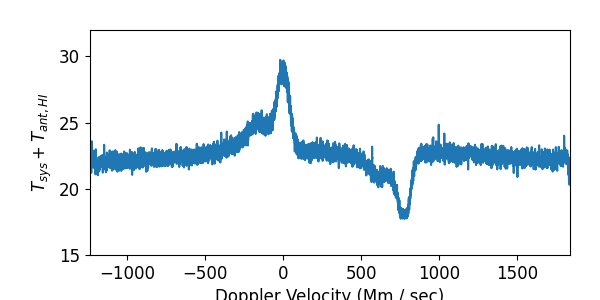
\includegraphics[width=.6\linewidth]{cass_vs_vel}
	\caption{...}
	\label{fig:cass_vs_vel}
\end{figure}

\

\textcolor{red}{What was the point of fitting anything to a Gaussian? Furthermore, include the parameters of the two Gaussians that you have here put forward.}

\begin{figure}
\centering
	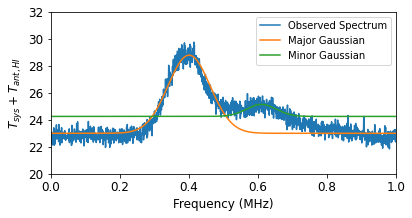
\includegraphics[width=.6\linewidth]{gauss}
	\caption{The minor Gaussian, I cannot say for sure it is there. The major one, by contrast, looks pretty neat.}
	\label{fig:gauss}
\end{figure}

A quick calculation: take the average of all null spacings.

Plot: data (position versus null), fit line, error bars...

\section{Conclusions}

\quad \quad 

% This would be a good place to talk about the difference between open and shorted waveguides, and perhaps even the significance to VSWR

\section{Acknowledgments}

\quad \quad \textcolor{red}{You have to remedy your complete ignorance of BibTex}

\end{document}
